\documentclass[11pt,a4paper]{article}
\usepackage[T1]{fontenc}
\usepackage[utf8]{inputenc}
\usepackage{lmodern}
\usepackage{amsmath,amssymb,amsthm,mathtools,mathrsfs}
\usepackage{graphicx,float,xcolor,multicol}
\usepackage[shortlabels]{enumitem}
\usepackage[margin=27mm]{geometry}
\usepackage{microtype,needspace,placeins}
\usepackage{tikz,tikz-cd}
\usetikzlibrary{arrows.meta,calc,positioning,patterns,decorations.pathreplacing}
\usepackage[colorlinks=true,linkcolor=teal,urlcolor=teal,citecolor=teal]{hyperref}
\setlength{\parindent}{0pt}
\setlength{\parskip}{.6em}
\setcounter{secnumdepth}{0}
\allowdisplaybreaks
\raggedbottom
\providecommand{\cross}{\times}
\DeclareUnicodeCharacter{2020}{\ensuremath{\dagger}}
\DeclareMathOperator{\supp}{supp}
\DeclareMathOperator*{\esssup}{ess\,sup}
\providecommand{\chapter}{\section}
\newenvironment{tool}[2]{\subsection*{Tool #1 --- #2}}{}
\newcommand{\ToolRef}[1]{Tool #1}
\newcommand{\FigureTag}[2]{\textit{Figure #1}}
\newcommand{\Result}[1]{\subsection*{#1}}
\newcommand{\Application}[1]{\subsubsection*{Application\if\relax\detokenize{#1}\relax\else\space--- #1\fi}}
\newcommand{\ProofHeading}{\par\textit{Proof.}\space}
\newcommand{\ProofOf}[1]{\par\textit{Proof of #1.}\space}
\newcommand{\RemarkHeading}{\par\textbf{Remark.}\space}
\newcommand{\NoteHeading}{\par\textbf{Note.}\space}
\newcommand{\ExerciseHeading}{\par\textbf{Exercise.}\space}

\graphicspath{{figures/mcmullens-surgery/}}
\begin{document}
\section*{McMullen's Surgery I: Ideal Boundaries and the Gluing Lemma}
% BLOG-CONTENT-BEGIN
\begin{center}
\emph{McMullen's Surgery:} Part I \(\,\cdot\,\)
\BlogPost{mcmullens-surgery}{Part II} \(\,\cdot\,\)
\BlogPost{mcmullens-surgery-finite-symmetry}{Part III}
\end{center}

Let $f$ be a rational map of degree at least $2$ on $\hat{\mathbb{C}}$, and $\text{Aut}(f)$ the group of M\"obius transformations commuting with $f$. Given any such transformation $M$, for each $n$, $M$ permutes the finitely many periodic points of order $n$. Choose $n$ so that this set has at least three distinct points. The induced action of $\text{Aut}(f)$ on this finite set is faithful, since a M\"obius transformation fixing three points is the identity. Therefore, $\text{Aut}(f)$ is a finite group. We shall now attempt to loosen the regularity and see if the finiteness can be retained. To begin with, let $\text{Mod}(f)$ denote the group of isotopy classes of quasiconformal maps commuting with $f$. It can be shown that regardless of the group being infinite and complicated, all its finite subgroups can be realized as subgroups of $\text{Aut}(g)$ for some deformation $g$ of $f$. So, we pull our necks a bit more to the surface and ask what about the group $\text{Mod}(J, f)$, the group of quasiconformal maps commuting with $f$ only on its Julia set? Yet again, it can be shown that if the Julia set is connected and carries no invariant line field, then $\text{Mod}(J, f)$ is a finite group. The proof of the former claim uses Nielsen realization for Riemann surfaces and is done in \cite{mcmullen1988automorphisms}, \cite{mcmullen1998quasiconformal} and \cite{imayoshi2012introduction}; the latter claim will be our focus here. Let us define certain objects before proceeding further.

    \subsection*{Definition 6.1}{(Invariant Line Field on the Julia Set)}: A line field on the Julia set $J(f)$ of $f$ is a measurable Beltrami differential $\mu(z)$, supported on a positive area subset of $J(f)$, with $|\mu(z)|=1$ almost everywhere on its support. It is said to be invariant if $f^*\mu = \mu$.


    \subsection*{Definition 6.2}{(Stable Conjugacy)}: Let $f$, $g$ be two rational maps, and $F$, $G$ be two closed subsets of the Riemann sphere such that $f(F) = F$ and $g(G) = G$. A map $\phi:\hat{\mathbb{C}} \rightarrow \hat{\mathbb{C}}$ determines a stable conjugacy $(F, f) \sim (G, g)$ if
    \begin{enumerate}
        \item $\phi$ is quasiconformal on $\hat{\mathbb{C}}$.
        \item $\phi(F) = G$.
        \item $\phi \circ f(z) = g\circ \phi(z)$ for all $z\in F$.
    \end{enumerate}

    We say that two maps $\phi$, $\psi$ determine the same stable conjugacy if they are isotopic through maps satisfying the three aforementioned conditions. The group of self stable conjugacies $(F, f)$ is denoted by $\text{Mod}(F, f)$.


    We shall study the finiteness of the object $\text{Mod}(K, f)$, the group of quasiconformal maps commuting with $f$ on $K$ (a forward invariant component of $J(f)$). Our main goal will be proving the following.

    \subsection*{Theorem 6.3}{(Commuting Deformations on Julia Sets)}: Let $K$ be a component of the Julia set of $f$ (which is assumed to have more than one point) such that $f(K) = K$. Then:
    \begin{enumerate}
        \item There exists a rational map $g$ with Julia set $J(g)$ and a stable conjugacy $\phi:(K,f)\sim (J(g), g)$ that determines an isomorphism $\text{Mod}(K, f) \cong \text{Mod}(J(g), g)$.
        \item If $K$ above carries no invariant line field, then $g$ can be chosen so that $\text{Mod}(J(g), g) \cong \text{Aut}(g)$. In particular, $\text{Mod}(K, f)$ is a finite group.
    \end{enumerate}


    Now the finiteness above is only for stable conjugacies on certain components of the Julia set. In particular, one can easily deduce from the theorem above that if the Julia set is connected and admits no invariant line field then $\text{Mod}(J(f), f)$ is a finite group. It has been conjectured that the hypothesis demanding the non-existence of invariant line fields on $J(f)$ can be dropped.

    \subsection*{Conjecture 6.4}: For any nonaffine rational map $g$ with connected Julia set $J$, $\text{Mod}(J, g)$ is a finite group.


    At the end, we shall briefly touch upon this conjecture for the case of exposed critical points. Let us now begin the proof of Theorem $6.3$

    \subsection*{Proposition 6.5}{(Rickman's Lemma)}: Let $\phi:\hat{\mathbb{C}}\rightarrow\hat{\mathbb{C}}$ be a homeomorphism and $R\subset\hat{\mathbb{C}}$ an open region. If $\phi\big|_R$ is $K$-qc and $\phi\big|_{\hat{\mathbb{C}}\backslash R} = \text{Id}\big|_{\hat{\mathbb{C}}\backslash R}$, then $\phi$ is quasiconformal \cite{mcmullen1988automorphisms}.



    This surgery, unlike the preceding two, cuts and pastes along ideal boundaries rather than topological boundaries \cite{mcmullen1988automorphisms,branner2014quasiconformal}. So, we begin by formulating an appropriate analogue of Rickman's lemma to help us formulate a mechanism with which we can glue certain deformed objects.

    \subsection*{Definition 6.6}{(Ideal Boundary of a Disc)}: By a disk $U \subset \hat{\mathbb{C}}$ we mean a simply connected domain whose complement contains at least two points. For a disk $U$, the ideal boundary $I(U)$ is the set of all prime ends of $U$.

    \begin{figure}[H]\centering
    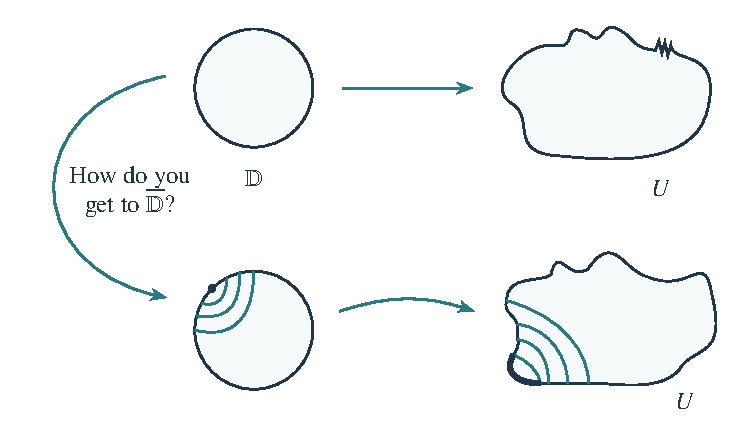
\includegraphics[width=12cm]{ms-fig-01.pdf}
    \FigureTag{MS1}{fig:ms-01}
    \end{figure}

    \begin{figure}[H]\centering
    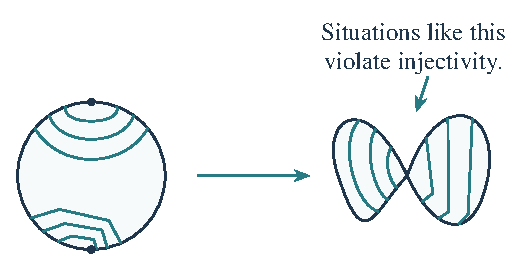
\includegraphics[width=11.5cm]{ms-fig-02.pdf}
    \FigureTag{MS2}{fig:ms-02}
    \end{figure}

    Given a proper holomorphic map $f:U\rightarrow V$ between discs $U$ and $V$, one obtains an induced map between their respective ideal boundaries. Indeed, consider the Riemann maps $R_U:U\rightarrow \mathbb{D}$ and $R_V:V\rightarrow \mathbb{D}$, and consider the composition $\hat{f} = R_V\circ f \circ R_U^{-1}: \mathbb{D}\rightarrow\mathbb{D}$, a proper holomorphic self map. Using reflection across $\mathbb{S}^1$, namely $z\mapsto 1/\bar z$, and the Schwarz Reflection Principle, one can extend the map to a real analytic map on $\mathbb{S}^1$. Since Riemann maps give homeomorphisms between $\mathbb{S}^1$ and the corresponding ideal boundaries, we have a map $\hat{f}:I(U)\rightarrow I(V)$. It doesn't make sense to call $\hat{f}$ real analytic intrinsically, but whenever we do so we invariably see it in these circle coordinates. Now with this in mind let us formulate an analogue of Rickman's lemma.

    \subsection*{Proposition 6.7}: Let $U$ be a disk. We have the following:
    \begin{enumerate}
        \item Let $\phi:\overline{U}\rightarrow\overline{U}$ be a homeomorphism. If $\phi\big|_{\partial U} \equiv \text{Id}\big|_{\partial U}$, then $\phi\big|_{I(U)} \equiv \text{Id}\big|_{I(U)}$.
        \item Let $\phi:U\rightarrow U$ be a quasiconformal map. If $\phi\big|_{I(U)} \equiv \text{Id}\big|_{I(U)}$, then $\phi$ extends quasiconformally by the identity to $\hat{\mathbb{C}}$ and $\phi\big|_{\partial U} \equiv \text{Id}\big|_{\partial U}$.
    \end{enumerate}


    \textit{Proof.}: $(1)$ $\phi$ is continuous on $\overline{U}$ implies $\phi$ is uniformly continuous as $\overline{U}$ is compact. Let $\{C_n\}_n$ be a sequence of crosscuts. As $\phi$ is a homeomorphism and $\text{diam}(C_n) \rightarrow 0$, uniform continuity ensures that if $\{C_n\}_n$ defines a prime end, then so does $\{\phi(C_n)\}_n$. Let $U_1 \supset U_2 \supset \cdots \supset U_n \supset \cdots$ be the prime end corresponding to $\{C_n\}$. Then an easy consequence of Jordan Curve Theorem would tell us that $C_l \subset U_k$ for all $l>k$.\\
    Set $Q_k$ to be the quadrilateral bounded by $C_k\cup C_{k+1}$ in $U$ for large $k$. Fix $n$. Suppose there exists an increasing sequence $\{k_i\}_i$ such that $Q_{k_i}$ and $\phi(Q_{k_i})$ belong to different components of $U\backslash C_n$. After passing to a subsequence, choose $x_{k_i}\in Q_{k_i}$ with $x_{k_i}\rightarrow x\in\mathcal{E}\subset\partial U$, where $\mathcal{E}$ is the impression of the prime end.\\
    As $\phi$ is uniformly continuous, $\phi(x_{k_i}) \rightarrow \phi(x) = x$ ($\phi$ is identity on $\partial U$), but this forces $\phi(x_{k_i})$ and $x_{k_i}$ to eventually land in the same component of $U\backslash C_n$. Contradiction.\\
    Thus, for every fixed $n$, $\phi(U_k)\subset U_n$ for all sufficiently large $k$. Applying the same argument to $\{\phi(U_k)\}_k$ and $\phi^{-1}$ shows that the two chains define the same prime end.

    (2) Observe that if $\phi$ is identity on the ideal boundary of $U$ then $\sup_{z\in U}d_U(\phi(z),z) < \infty$, where $d_U$ is the Poincar\'e distance on the hyperbolic surface $U\cong\mathbb{D}$; this is the bounded-displacement property of a quasiconformal self-map of the disk with identity boundary values \cite{mcmullen1988automorphisms}. Suppose $\sup_{z\in U}d_U(\phi(z),z) < K$. Given any $\{x_k\}_k$ such that $x_k\rightarrow x \in \partial U$, note that $\phi(x_k) \in B_K(x_k)$, the ball of radius $K$ around $x_k$. Since $\overline{U}$ is compact in $\hat{\mathbb{C}}$ and $U$ is hyperbolic, we know that $B_K(x_k) \rightarrow x \in \partial U$. In particular, $\phi(x_k) \rightarrow x$ $\implies$ $\phi$ extends to $\partial U$ continuously and $\phi\big|_{\partial U} \equiv \text{Id}\big|_{\partial U}$. A direct application of Rickman's lemma now completes the proof.

    \begin{figure}[H]\centering
    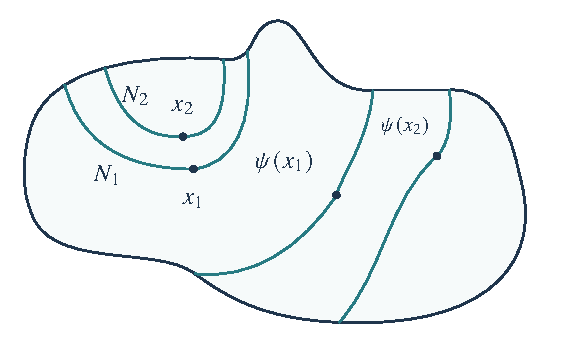
\includegraphics[width=12cm]{ms-fig-13.pdf}
    \FigureTag{MS13}{fig:ms-13}
    \end{figure}


    \subsection*{Proposition 6.8}
    Let $\phi$, $\psi: \overline{U} \rightarrow \overline{V}$ be homeomorphisms where $U$ and $V$ are discs, $K$-qc on $U$ and equal on $\partial U$. Then there exists an isotopy connecting $\phi$ to $\psi$ through $K^3$-qc maps all agreeing on $\partial U$.


    \textit{Proof.}: Let $\alpha = \psi^{-1}\circ \phi: U \rightarrow U$. Then $\alpha$ is $K^2$-qc and is identity on $I(U)$ by the previous proposition. We construct $\alpha_t$ connecting $\alpha$ to the identity map through homeomorphisms enjoying the two properties that $\alpha$ does. Uniformize $U$ and bring the identity in radially from the boundary of the unit disk, as in \cite{mcmullen1988automorphisms}; this gives the required isotopy through $K^2$-qc maps. Push it to $U$ and note that the desired isotopy is given by $\phi_t = \psi\circ \alpha_t$. Its maps are $K^3$-qc and agree on $\partial U$.


    \subsection*{Corollary 6.9} If $K$ is connected and periodic points of $f$ are dense in $K$, then any $[\phi]$ in $\text{Mod}(K, f)$ is uniquely determined by its values on $K$.


    \textit{Proof.}: Let's now construct a stable conjugacy taking $\phi$ to $\text{Id}$, given that $\phi = \text{Id}$ on $K$. Here, $K$ is compact connected. Let $\hat{\mathbb{C}}\backslash K = \sqcup_{\alpha}U_{\alpha}$, then $U_{\alpha}$'s are simply connected. Indeed, let $\gamma$ be a loop in $U_{\alpha}$, then as $\gamma \cap K = \varnothing$, one can construct a polygonal region $\tilde{\gamma}$ such that $K$ and $\gamma$ belong to different components of $\hat{\mathbb{C}}\backslash \tilde{\gamma}$. Now the claim is a simple consequence of the Jordan Curve Theorem: if $\gamma \subset \text{Int}(\tilde{\gamma})$, then $\text{Int}(\tilde{\gamma})\subseteq U_{\alpha}$. By the previous propositions, on each disk in the complement of $K$ there is an isotopy connecting $\phi$ to the identity through quasiconformal maps which are identity on $K$. The dilatation of the intervening maps is bounded by $K(\phi)^3$ (independent of the disk). By Proposition $6.5$ the time $t$ maps in each disk piece together to form a quasiconformal map of the whole Riemann sphere. Thus, $[\phi] = [\text{Id}]$ in $\text{Mod}(K,f)$.


    \subsection*{Definition 6.10}{(Ideal Boundary of $K$)}: We define $I(K)$, the ideal boundary of a given infinite continuum $K$, to be the union of the ideal boundaries of the disks in the complement of $K$. (Note: In what's to follow $K$ shall be a forward invariant component of $J(f)$ unless otherwise stated).



    \begin{figure}[H]\centering
    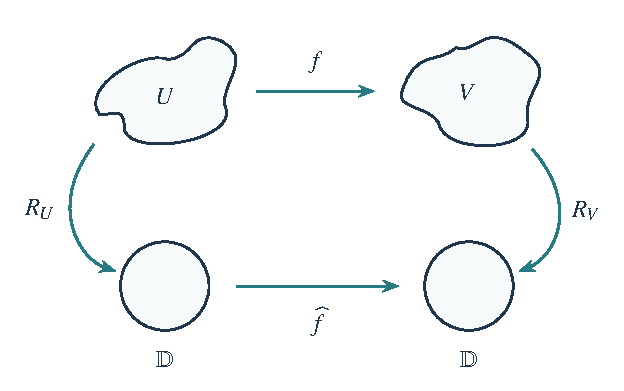
\includegraphics[width=10cm]{ms-fig-03.pdf}
    \FigureTag{MS3}{fig:ms-03}
    \end{figure}

    \begin{figure}[H]\centering
    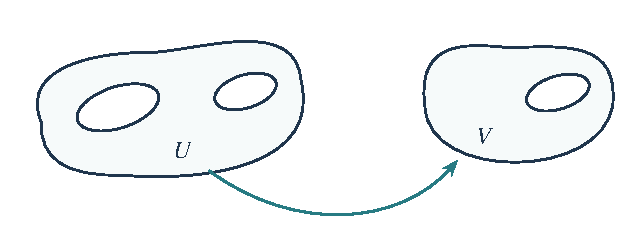
\includegraphics[width=12cm]{ms-fig-04.pdf}
    \FigureTag{MS4}{fig:ms-04}
    \end{figure}

    If $f$ is quasirational (i.e. quasiconformally conjugate to a rational function on $\hat{\mathbb{C}}$), then $f$ induces a map $\hat{f}: I(K) \rightarrow I(K)$ which is quasisymmetrically conjugate to a real analytic map. Indeed, firstly assume $f$ to be rational. Since $\text{deg}(f) < \infty$, $f^{-1}(K)$ consists of $K$ and finitely many other components. Let $U$ be a component of $\hat{\mathbb{C}}\backslash K$, and let $U'$ be the component of $U\backslash f^{-1}(K)$ whose closure contains $\partial U$. Then $f$ carries $U'$ properly to a component $V$ of $\hat{\mathbb{C}}\backslash K$. In Riemann-map coordinates for $U$ and $V$, the map $f$ carries a neighbourhood of $\mathbb{S}^1$ to a neighbourhood of $\mathbb{S}^1$. By the Schwarz Reflection Principle it extends across the circle and induces a real analytic map $\hat{f}:I(U)\rightarrow I(V)$. If $f$ were now only quasirational, then the induced map on the ideal boundary of $K$ would be quasisymmetrically conjugate to a real analytic map.


    \begin{figure}[H]\centering
    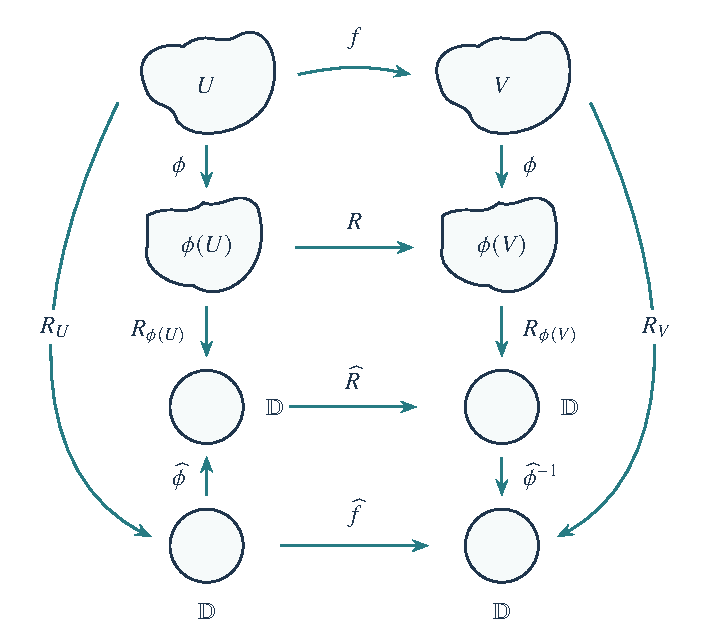
\includegraphics[width=10cm]{ms-fig-05.pdf}
    \FigureTag{MS5}{fig:ms-05}
    \end{figure}
    All surgery principles introduced so far are means to deform a rational map to another rational map, so for one to perform successive surgeries one must constantly convert one's results back to something rational. The Gluing Lemma introduced below as a substitute for Rickman's Lemma will allow us to bypass that, thereby standing as a surgery principle in its own right for quasirational maps.

    \subsection*{Definition 6.11}{(Compatibility of Maps on the Ideal Boundary)}: Let $K$ be a non-degenerate invariant continuum such that $f^{-1}(K)$ consists of $K$ and finitely many other disjoint components. Let $U$ and $V$ be components of $\hat{\mathbb{C}}\backslash K$ so that $\hat{f}:I(U) \rightarrow I(V)$ as described above is the induced map. Let $B$ denote a Blaschke product mapping $\overline{\mathbb{D}}$ onto itself \cite{garcia2018finite}. We say $f$ and $B$ are compatible on the ideal boundary of $U$ via quasiconformal maps $\phi_U:U\rightarrow \mathbb{D}$ and $\phi_V:V\rightarrow \mathbb{D}$, if the induced maps $\hat{\phi}_U: I(U) \rightarrow \mathbb{S}^1$ and $\hat{\phi}_V: I(V) \rightarrow \mathbb{S}^1$ define a quasisymmetric equivalence between $\hat{f}:I(U) \rightarrow I(V)$ and the restriction of $B$ to the unit circle, as shown in the following commutative diagram:

    $$\begin{tikzcd}[column sep = large, row sep = large]
        I(U)
        \arrow[d, "\hat{\phi}_U"']
        \arrow[r, "\hat{f}"]
        &
        I(V)
        \arrow[d, "\hat{\phi}_V"]
        \\
        \mathbb{S}^1
        \arrow[r, "B"']
        &
        \mathbb{S}^1
        \\
        \end{tikzcd}$$



    We are now ready to state and prove the Gluing Lemma.

    \subsection*{Lemma 6.12}{(Gluing Lemma)}: In the setup of the definition above suppose that:
    \begin{enumerate}
        \item either $I(U)$ is a fixed component of $I(K)$ under the map $\hat{f}:I(K)\rightarrow I(K)$, and $\phi_U=\phi_V=\phi$,
        \item or $I(U)$ is non-recurrent under $\hat{f}$, so that $\hat{f}^{\circ n}(I(U)) \cap I(U) = \varnothing$ for all $n>0$.
    \end{enumerate}

    Assume $f$ and $B$ are compatible on $I(U)$ via maps $\phi_U$ and $\phi_V$. Then the map

    $$g(z):= \begin{cases}
        f(z), &\quad\text{if}  z \notin U\\
        \phi_V^{-1}\circ B\circ \phi_U(z) &\quad\text{if}   z\in U\\
        \end{cases}$$

    is quasirational.


    \textit{Proof.}: Consider locally the branch of $f^{-1}\circ g$ that agrees with the identity outside $U$. It is the identity outside $U$ and quasiconformal inside $U$. It also induces the identity map on the ideal boundary since $\hat{f} = \hat{\phi}_V^{-1}\circ B\circ\hat{\phi}_U = \hat{g}:I(U)\rightarrow I(V)$. Using Proposition $6.5$ we note that $f^{-1}\circ g$ is locally quasiconformal. By composing with $f$ we obtain that $g$ is locally quasiconformal except on neighbourhoods of the branch points. Hence, $g$ is quasiregular. The dilatation of $g$ is bounded by the maximum of $K(f)$ and $K(\phi_U)\cdot K(\phi_V)$.\\

    \begin{figure}[H]\centering
    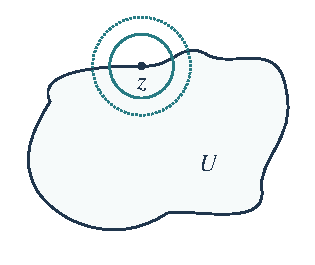
\includegraphics[width=6cm]{ms-fig-07.pdf}
    \FigureTag{MS7}{fig:ms-07}
    \end{figure}

    \begin{figure}[H]\centering
    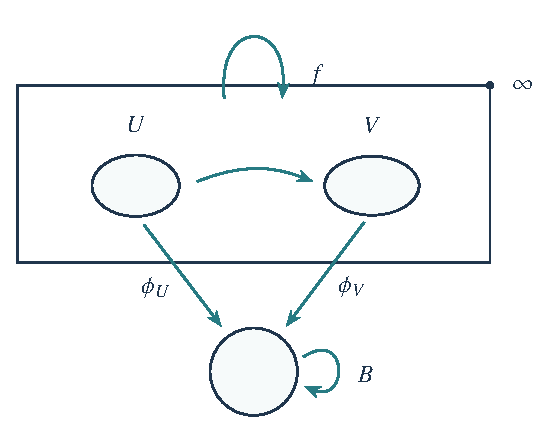
\includegraphics[width=10cm]{ms-fig-11.pdf}
    \FigureTag{MS11}{fig:ms-11}
    \end{figure}
    If $I(U)$ is a fixed component of $\hat{f}$, then $g(U) = U$ and $g^{\circ n}\big|_U = \phi^{-1}\circ B^{\circ n}\circ \phi$. Hence, we have $K(g^{\circ n}) \leq K(\phi)^2$ on $U$. If $z \notin U$, it may have several iterates in $\hat{\mathbb{C}}\backslash U$ before falling into $U$. Hence, $K(g^{\circ n}) \leq K(f^{\circ n})\cdot K(\phi)^2\leq K\cdot K(\phi)^2$, where $f$ is quasirational so that $K(f^{\circ n}) \leq K$ for all $n$ and some $K \geq 1$ (by Sullivan's Straightening Theorem). Hence, $g$ is quasirational.\\
    In the non-recurrent case, the dilatation is $K(g^{\circ n}) \leq K\cdot K(\phi_U)\cdot K(\phi_V)$, since no orbit can pass through $U$ more than once.


    \subsection*{Corollary 6.13} In the setup above, suppose $U_0 = U_p$, and $U_1, U_2,\ldots, U_{p-1}$ are components of $\hat{\mathbb{C}}\backslash K$ such that $\hat{f}^{\circ j}(I(U_0)) = I(U_j)$ for $0\leq j\leq p-1$. Set $\phi_p=\phi_0$. For $j = 0, 1, \ldots, p-1$, let $B_j$ be Blaschke products compatible with $f\big|_{U_j}$ on the ideal boundary via the maps $\phi_j$ and $\phi_{j+1}$. Then the map
    $$g(z):= \begin{cases}
        f(z), &\quad\text{if}  z \notin \bigcup_{j=0}^{p-1}{U_j}\\
        \phi_{j+1}^{-1}\circ B_j\circ \phi_j(z) &\quad\text{if}   z\in U_j\\
        \end{cases}$$

        is quasirational.


    \textit{Proof.}: Note that $g^{\circ p}$ is quasiconformally conjugate to a Blaschke product of degree $d = \prod_{j=0}^{p-1}{\text{deg}(B_j)}$ on any of the $U_j$'s. Since the cycle contains only finitely many $U_j$, this bound is uniform on their union, while the original bound for $f$ applies off the cycle. Therefore, $K(g^{\circ n})$ is uniformly bounded forcing $g$ to be quasirational by Straightening Theorem.

    \begin{figure}[H]\centering
    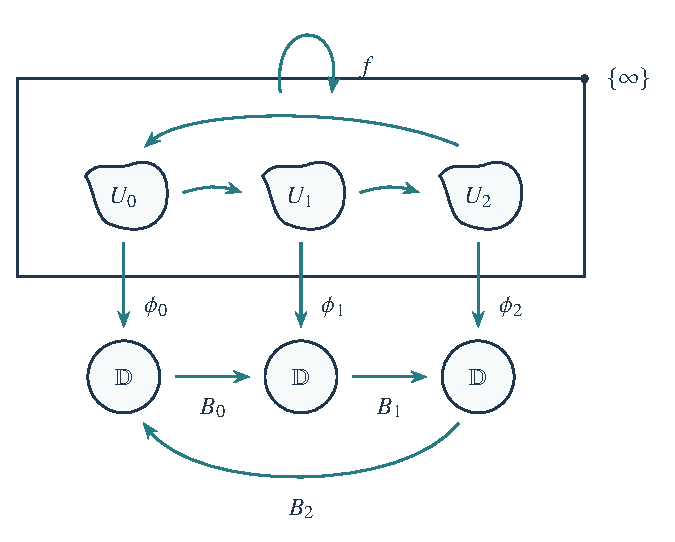
\includegraphics[width=11.5cm]{ms-fig-14.pdf}
    \FigureTag{MS14}{fig:ms-14}
    \end{figure}

\begin{center}
\BlogPost{mcmullens-surgery}{Continue to Part II: Rigid Models and a Julia Component}
\end{center}
% BLOG-CONTENT-END
\bibliographystyle{amsalpha}
\bibliography{tools/profiles/surgeries/MSc_Dissertation}
\end{document}
